% Tikz File 'model640.tex'
\documentclass{standalone}

\usepackage{tikz} %Graphics
\usetikzlibrary{shapes.geometric, arrows}
\tikzstyle{title} = [text centered]
\tikzstyle{block} = [rectangle, rounded corners, minimum width=3cm, minimum height=1.5cm,text centered, draw=black, fill=blue!30]
\tikzstyle{conv} = [rectangle, rounded corners, minimum width=3cm, minimum height=1.5cm,text centered, draw=black, fill=blue!30]
\tikzstyle{batchnorm} = [rectangle, rounded corners, minimum width=3cm, minimum height=1cm,text centered, draw=black, fill=green!30]
\tikzstyle{relu} = [rectangle, rounded corners, minimum width=3cm, minimum height=1.5cm,text centered, draw=black, fill=orange!30]
\tikzstyle{maxpool} = [rectangle, rounded corners, minimum width=3cm, minimum height=1.5cm,text centered, draw=black, fill=red!30]
\tikzstyle{arrow} = [thick,->,>=stealth]

%\usetikzlibrary{...}
\begin{document}
	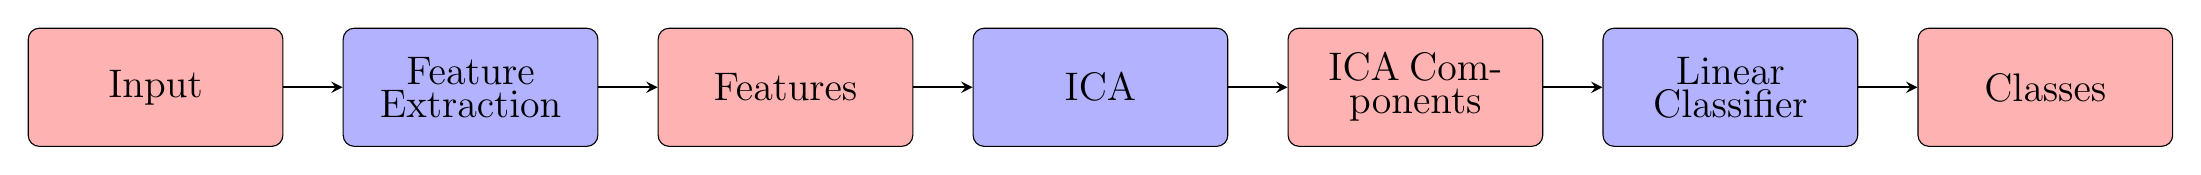
\begin{tikzpicture}[node distance=4cm]
		%\node (decomp) [title] { Initial Classifier };
		\node (l0) [maxpool, xshift=11mm, text width=3cm] {\Large Input};			
		\node (l1) [conv, right of = l0, text width=3cm] {\Large Feature Extraction};
		\node (l2) [maxpool, right of=l1, text width=3cm] {\Large Features};
		\node (l3) [conv, right of=l2, text width=3cm] {\Large ICA};
		\node (l4) [maxpool, right of=l3, text width=3cm] {\Large ICA Components};
		\node (l5) [conv, right of=l4, text width=3cm] {\Large Linear Classifier};
		\node (l6) [maxpool, right of=l5, text width=3cm] {\Large Classes};
		
		\draw [arrow] (l0) -- (l1);		
		\draw [arrow] (l1) -- (l2);
		\draw [arrow] (l2) -- (l3);
		\draw [arrow] (l3) -- (l4);	
		\draw [arrow] (l4) -- (l5);	
		\draw [arrow] (l5) -- (l6);	
			
\end{tikzpicture}
\end{document}
